\documentclass[fleqn,10pt]{wlscirep}
\usepackage[utf8]{inputenc}
\usepackage[T1]{fontenc}
\usepackage{float}
\usepackage{indentfirst}
\title{DEEP LEARNING FOR SKIN LESION SEGMENTATION: A REVIEW}

\author[1,*]{Duy Hung BUI}
\author[2,+]{Huy Hoang VU}

\affil[1]{202412987, Hanoi University of Science and Technology, Hanoi, Vietnam}
\affil[2]{202412982, Hanoi University of Science and Technology, Hanoi, Vietnam}

%\keywords{Keyword1, Keyword2, Keyword3}

\begin{abstract}

    Accurate skin lesion segmentation is a critical prerequisite for Computer-Aided Diagnosis (CAD) systems for melanoma. Over the past decade, Deep Learning architectures have become the gold standard; however, their effective deployment requires sophisticated optimization strategies to address artifacts and fuzzy boundaries. This paper presents a comprehensive review of computational techniques, categorized by their optimization objectives. We first discuss foundational Convolutional Neural Network (CNN) optimization strategies, ranging from structural refinements (Improved U-Net, FCN-based U-Net) and receptive field expansion (DeepLab), to automated hyperparameter tuning via Bayesian SegNet and attention mechanism integration (Attention Gates, CBAMSNet). Subsequently, we analyze the shift towards global context modeling with Hybrid Transformers (FAT-Net), which address the local inductive bias of CNNs. Finally, we evaluate the emerging trend of 2024: State Space Models (Mamba). Specifically, hybrid architectures such as AC-MambaSeg and VM-SwinUnet are critically analyzed to demonstrate their ability to balance segmentation accuracy with linear computational efficiency ($O(N)$). The review also highlights the role of Generative Adversarial Networks (GANs) in data augmentation and boundary refinement, providing a holistic perspective for developing next-generation clinical diagnostic systems. 

\end{abstract}
\begin{document}

\flushbottom
\maketitle
% * <john.hammersley@gmail.com> 2015-02-09T12:07:31.197Z:
%
%  Click the title above to edit the author information and abstract
%
\thispagestyle{empty}
\section*{Introduction}
    The skin serves as a vital interface between the human body and the external environment, governing essential functions such as temperature regulation and fluid retention. Despite its resilience, the skin is prone to a multitude of pathologies. It is estimated that there are over 3,000 distinct types of dermatological disorders, making skin diseases one of the most prevalent and diagnostically challenging health concerns worldwide. Global Cancer Statistics 2020 states that fatal skin lesions claim thousands of lives annually \cite{GlobalCancer}. More precisely, skin cancer ranks as the third most common human malignancy, with melanoma being its most aggressive and lethal form. Epidemiological data indicates a rapid surge in melanoma incidence over the last three decades. Notably, statistical projections estimated approximately 96,480 new diagnoses in the United States in 2019 \cite{Melanoma}.

    Dermoscopy, a non-invasive imaging technique, has improved diagnostic accuracy; however, manual interpretation of dermoscopic images is labor-intensive, subjective, and heavily dependent on the clinician's expertise. Consequently, CAD systems have become indispensable tools in clinical dermatology. Within the CAD pipeline, skin lesion segmentation, the process of accurately delineating the lesion boundary from the surrounding healthy skin, is the most critical prerequisite.
    
    Accurate recognition of melanoma presents significant challenges due to several inherent complexities. Firstly, the low contrast between lesions and the surrounding healthy skin often creates ambiguous boundaries \cite{FCN}, \cite{GAN}, \cite{Deeplab}.  Secondly, high variability in patient-specific attributes, ranging from skin pigmentation and texture to lesion morphology, complicates the detection process \cite{UNet}, \cite{GAN}, \cite{Deeplab}, \cite{Transformer}. Furthermore, image quality is frequently compromised by various artifacts, including body hair, specular reflections, air bubbles, shadows, and inconsistent lighting conditions \cite{FCN}, \cite{UNet}, \cite{GAN}, \cite{Transformer}. Thirdly, the scarcity of high-quality annotated training data poses a severe constraint on the model's generalization capability. Fourthly, the class imbalance problem, where the lesion area is disproportionately smaller than the background, significantly impedes segmentation performance. Notably, these aforementioned occlusions and artifacts are pervasive in standard public dermoscopic datasets. Figure 1 visually exemplifies these impediments, highlighting the complexity involved in precise boundary delineation.

        \begin{figure}[H]
        \centering
        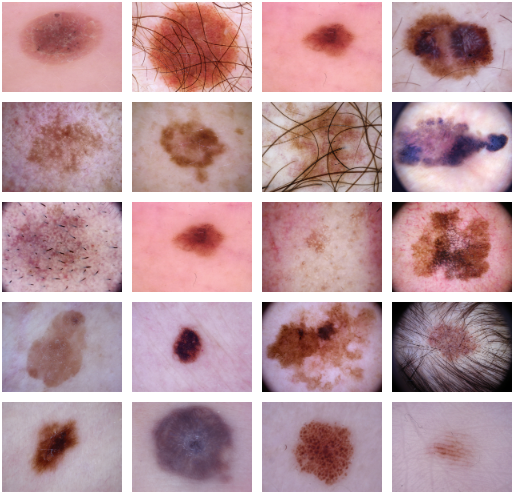
\includegraphics[width=0.6\linewidth]{ISIC2018.png}
        \caption{Dermoscopic images of some of the skin diseases from the ISIC 2016 dataset \cite{Skin}.}
        \label{fig:skindiseases}
        \end{figure}

    Early Deep Learning approaches, particularly Fully Convolutional Networks (FCN) and U-Net, established a strong baseline but often struggled with complex lesion heterogeneity. Consequently, recent research has moved beyond "vanilla" architectures, focusing instead on optimizing foundational models. Significant efforts have been made to refine structural designs (Improved U-Net), automate hyperparameter tuning (Bayesian SegNet), and integrate attention mechanisms (Attention Gates, CBAMSNet) to enhance feature selection. Despite these optimizations, CNN-based methods remain inherently limited by their local receptive fields, failing to capture long-range semantic dependencies effectively.

    To bridge this gap, Vision Transformers (ViTs) and hybrid architectures like FAT-Net were introduced, leveraging self-attention to model global context. However, the quadratic computational complexity ($O(N^2)$) of Transformers poses a barrier to deployment on resource-constrained clinical devices. This trade-off has catalyzed the emergence of State Space Models (Mamba) in 2024. Offering the global modeling capability of Transformers with the linear efficiency ($O(N)$) of CNNs, Mamba represents a paradigm shift in medical image analysis.

    This paper provides a systematic review of these computational techniques. Unlike chronological surveys, we categorize methods based on their optimization strategies: from data augmentation via Generative Adversarial Networks (GANs) and structural optimizations of CNNs, to the global context modeling of Transformers, and finally, the efficiency-driven era of Hybrid Mamba Architectures (e.g., AC-MambaSeg, VM-SwinUnet). Through this analysis, we aim to identify the most promising directions for future real-time diagnostic systems. To visualize this landscape, \textbf{Fig. \ref{fig:taxonomy}} presents the taxonomy of the computational techniques reviewed in this study.
        \begin{figure}[H]
        \centering
        \includegraphics[width=0.65\linewidth]{Taxonomy.jpg}
        \caption{Taxonomy of computational techniques for skin lesion segmentation utilized in this survey, categorizing methods from foundational CNNs to state-of-the-art Hybrid Mamba architectures.}
        \label{fig:taxonomy}
        \end{figure}
\section*{The Computational Pipeline \& Data Preparation}
    The quality of input data plays a decisive role in the performance of deep learning models, adhering to the fundamental principle of "Garbage In, Garbage Out." particularly in dermatological analysis, the presence of extraneous artifacts and severe class imbalance necessitates sophisticated computational strategies before the primary segmentation stage.

    \subsection*{Artifact Removal and Normalization}
        Dermoscopic images are frequently compromised by artifacts such as body hair, gel bubbles, ruler markers, and uneven illumination, which can obstruct lesion boundaries and mislead feature extraction. To mitigate these issues, standard pre-processing pipelines are employed to standardize the input data. 

        Artifact Removal: Hair occlusion is the most common impediment. The DullRazor algorithm is the standard computational approach for this task. It operates by identifying dark hair structures using generalized grayscale morphological closing operations and subsequently replacing the occluded pixels with values interpolated from the surrounding non-occluded tissue.

        Color Normalization: Since dermoscopic images are acquired using various devices under different lighting conditions, color inconsistency can hinder model convergence. Techniques such as Shades of Gray or Gray World algorithms are utilized to correct the illumination and normalize the color distribution, ensuring that the model learns features based on the lesion's pathology rather than lighting variations.

    \subsection*{Advanced Data Augmentation Strategy via GANs}
        A critical bottleneck in training medical image segmentation models is data scarcity and class imbalance. Malignant melanoma samples are often significantly underrepresented compared to benign nevi in public datasets. Traditional augmentation techniques, such as geometric transformations (rotation, flipping) and color jittering, are widely employed to artificially increase the dataset size. However, these methods only produce variations of existing samples and fail to introduce sufficient diversity into the data distribution.To address this limitation GANs have emerged as a breakthrough approach. Fundamentally, a GAN architecture consists of two competing neural networks: a Generator ($G$) and a Discriminator ($D$). The Generator aims to synthesize realistic lesion images from random noise distributions, while the Discriminator acts as a binary classifier, attempting to distinguish between real clinical images and the synthetic ones produced by $G$. Through a min-max adversarial training process, the Generator progressively learns to produce high-fidelity lesion samples that capture the complex texture and color characteristics of real dermoscopic images, thereby enriching the training set.

            \begin{figure}[H]
            \end{figure}

        Beyond pure data synthesis, adversarial learning concepts have been successfully adapted to enhance segmentation performance directly. Dual Discriminators by Lei et al. \cite{GAN} deploy the segmentation network functions as the Generator, while two distinct Discriminators operate in parallel to supervise the output:

            \begin{itemize}
                \item A Global Discriminator ensures the overall structural consistency of the predicted mask.
                \item A Local Discriminator focuses specifically on the boundary details, enforcing sharpness at the lesion edges.
            \end{itemize}

        By subjecting the model to this "double scrutiny," the system learns to generate segmentation maps that are not only pixel-wise accurate but also visually consistent with expert annotations. This study demonstrates the versatile potential of GANs: acting as both a tool for data augmentation and a segmentation mechanism through adversarial loss.

    \section*{Optimizing Foundational CNN Architectures}

        While early CNNs marked a paradigm shift from manual feature extraction to automated learning, vanilla architectures often struggle with the specific challenges of dermoscopy, such as fuzzy boundaries and low contrast. Consequently, the first era of advancement was defined not merely by the application of CNNs, but by the rigorous optimization of foundational architectures. This section categorizes these computational improvements into three strategic domains: structural refinement, receptive field expansion, and attention-based feature selection.

    \subsection*{Structural and Hyperparameter Optimization}

        The transition from patch-based classification to pixel-wise segmentation was pioneered by FCNs. However, standard implementations often faced resolution loss during upsampling. To address this, FCN-based model optimized with a U-Net-like architecture \cite{FCN} was proposed. By adapting the FCN to learn end-to-end mappings while incorporating symmetric decoding paths, their approach effectively mitigates the loss of spatial information, demonstrating that FCNs can be structurally tuned to handle fine-grained lesion details.

        Parallel to structural design, the optimization of training hyperparameters remains a critical yet often overlooked aspect. The SegNet architecture, known for its memory-efficient use of pooling indices, is highly sensitive to parameter initialization. Sahin et al. \cite{SegNet} introduced a Bayesian Optimized SegNet, replacing manual trial-and-error with a probabilistic approach. By employing Bayesian optimization to automatically search for the optimal learning rate and momentum within a complex search space, they achieved superior segmentation accuracy compared to standard SegNet implementations. This highlights that computational optimization in the training phase is as vital as the architectural design itself.

        Furthermore, the standard U-Net, despite being the gold standard, can propagate noise through its skip connections. Liu et al. \cite{UNet} proposed an Improved U-Net, which refines the encoder-decoder path to better preserve boundary information. By optimizing the internal feature concatenation process, this improved variant significantly reduces false positives at the lesion periphery compared to the classic U-Net.

    \subsection*{Expanding Receptive Fields via Dilated Convolutions}

        A fundamental limitation of the aforementioned encoder-decoder models is the reduction of spatial resolution caused by pooling layers, which leads to coarse segmentation boundaries. To expand the receptive field without sacrificing resolution, Bagheri et al. \cite{Deeplab} proposed a hybrid framework integrating RetinaNet with DeepLab.

        The core innovation lies in the use of Atrous (Dilated) Convolution, which inserts holes (zeros) into the filters to enlarge the field of view. This allows the network to capture multi-scale contextual information—crucial for distinguishing large lesions from healthy skin—without increasing the number of parameters. Moreover, their approach goes beyond pure deep learning by incorporating a Graph-based refinement method in the post-processing stage. This hybrid pipeline, combining the object detection strength of RetinaNet, the semantic context of DeepLab, and the boundary precision of graph theory, exemplifies a sophisticated strategy to overcome the "local view" limitation of standard CNNs.

    \subsection*{Feature Selection with Attention and Dynamic Mechanisms}

        As network depth increases, the risk of learning redundant features (e.g., background artifacts like hair or gel) rises. To enable the network to "focus" on relevant regions, Attention Mechanisms were introduced.

        Arora et al. \cite{AttentionGates} integrated Attention Gates (AGs) into the U-Net architecture. Unlike hard attention which crops images, AGs employ soft attention to automatically learn weight coefficients that suppress irrelevant background regions while highlighting feature-rich lesion areas. This mechanism allows the model to inherently filter out artifacts without explicit pre-processing.

        Pushing the envelope of optimization further, recent works like CBAMSNet \cite{CBAMSNet} have combined attention with dynamic computation. This architecture integrates the Convolutional Block Attention Module (CBAM) to refine features along both channel and spatial dimensions. More importantly, it employs Omni-dimensional Dynamic Convolution (ODConv), where convolutional kernels are not static but dynamically adapt their weights based on the input image. This "dynamic" capability allows the network to be lightweight and computationally efficient while maintaining the flexibility to handle the high variability of skin lesion shapes.

\section*{The Shift to Global Context with Hybrid Transformers}

    While the optimized CNN architectures discussed in the previous section significantly improved boundary delineation, they remain bound by the inherent limitation of the convolution operation: the local receptive field. Even with dilated convolutions (as in DeepLab), CNNs struggle to capture long-range dependencies explicitly. In complex dermatological cases, where the diagnosis depends on the relationship between widely separated visual patterns, this local inductive bias becomes a bottleneck.

    To address this, the second era of computational techniques is defined by the integration of Transformers, leveraging the Self-Attention mechanism to model global context.

    \subsection*{Hybrid Architecture Strategy: The FAT-Net Case}

        Pure Transformers (like the original ViT) often suffer from localized feature loss due to patch partitioning and require massive datasets to converge. Therefore, the dominant strategy in medical imaging is the Hybrid Approach.

        A prime example is FAT-Net (Feature Adaptive Transformers) proposed by Wu et al. \cite{Transformer}. Instead of discarding the CNN entirely, FAT-Net employs a Dual-Encoder Strategy: 
        
            \begin{itemize} 
                \item A ResNet-50 backbone is used to extract high-resolution spatial features. 
                \item Transformer layers are embedded at the bottleneck to capture global semantic relationships.
            \end{itemize}

        The core computational innovation of FAT-Net is the Feature Adaptive Module (FAM). Recognizing that skin lesions often possess irregular shapes and varying sizes, the FAM utilizes channel attention to adaptively activate relevant feature maps while suppressing noise. Furthermore, to mitigate the high memory consumption typically associated with Transformers, the authors designed a Memory-Efficient Decoder. This structural optimization allows FAT-Net to achieve a superior Dice score compared to U-Net and Att-Unet, proving that combining the "local detail" of CNNs with the "global vision" of Transformers is more effective than using either in isolation.

\section*{Methods}

Topical subheadings are allowed. Authors must ensure that their Methods section includes adequate experimental and characterization data \cite{FCN}necessary for others in the field to reproduce their work.

\bibliography{sample}

\end{document}